\chapter{Results and discussion}

\section{Data exploration}
As described earlier in Chapter 3, the data for the experiments is from Twitter. It was extracted and pre-processed by \cite{preotiuc-pietro_automatically_2019} and further enhanced with the labels for complaint severity by \cite{jinModelingSeverityComplaints2021}. What follows are the key findings from the exploratory data analysis performed. Additionally, some minor differences in the distribution of the tweets across the domains are observed between the latest version of the dataset available in the public domain\footnote{\url{https://archive.org/details/complaint_severity_data}} and the distribution described in the original paper. Since the variations are minor (0.5 to 2\%), any potential impact on the model performance should be insignificant in the context of the objectives of the experiments. Refer \ref{sec: apdxa_fulldataset} for the full breakdown of the dataset used here.

\subsection{Domain and class distribution}
\begin{figure}[htb]
    \centering
    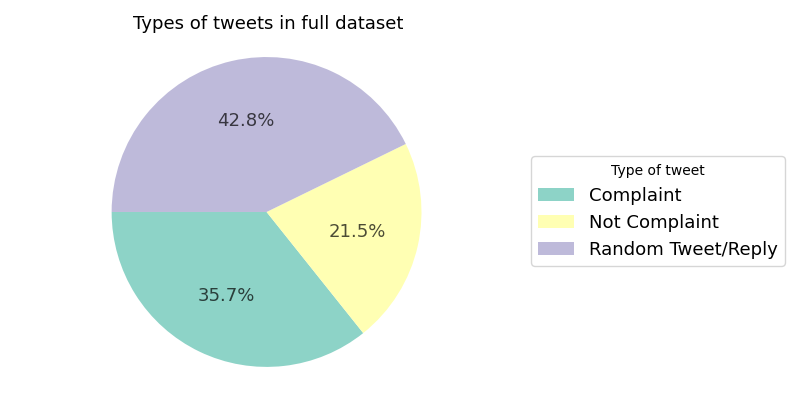
\includegraphics[width=9cm]{figures/compl_non_random_dist.png}
    \vspace*{-3mm}
    \caption{Illustrates the distribution of tweets categorised as 'complaints' and 'not complaints', with random 'tweets / replies' shown separately.}
    \label{fig: compl_non_random_dist}
\end{figure}


All tweets categorised as complaints are assigned the label \texttt{label:1}, while tweets that do not constitute complaints are assigned \texttt{label:0}. In terms of class distribution, the dataset is skewed towards 'not complaint' tweets, as depicted in Figure \ref{fig: compl_non_random_dist}, where \texttt{label:1} represents 35.7\% and \texttt{label:0} represents 64.3\% of the dataset. To ensure a more representative dataset, the authors of \cite{preotiuc-pietro_automatically_2019} introduced several random tweets and replies. This approach aligns with the real-world scenario where complaint-related posts form a smaller proportion within an organization's social media tweets and posts. Additionally, this strategy has the potential to enhance the model's ability to generalize effectively during the finetuning process.\\

\begin{figure}[htbp]
    \centering
    \captionsetup{font=small}
    \begin{subfigure}{0.49\textwidth}
        \centering
        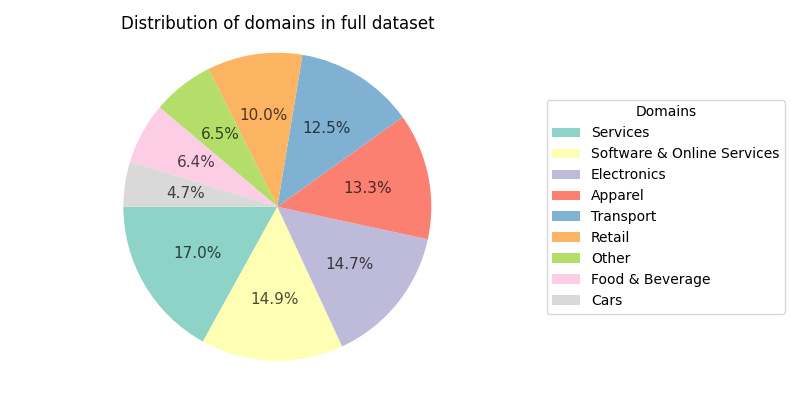
\includegraphics[width=\linewidth]{figures/domain_dist.png}
        \caption{Proportion of each domain}
        \label{fig: domain_dist_pct}
    \end{subfigure}
    \hfill
    \begin{subfigure}{0.49\textwidth}
        \centering
        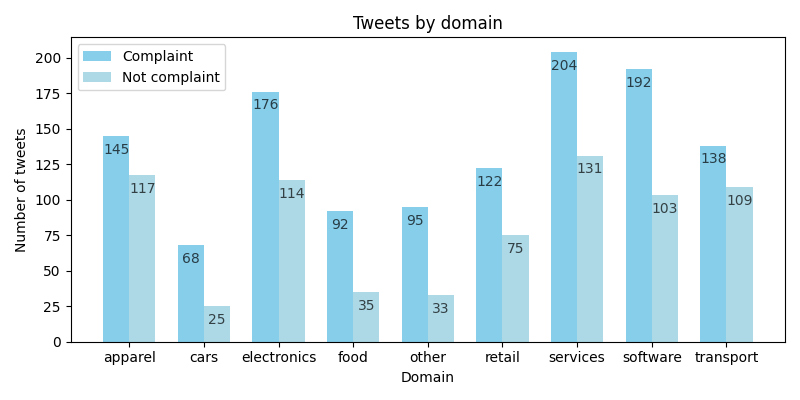
\includegraphics[width=\linewidth]{figures/domain_counts_bar_norandom.png}
        \caption{No. of tweets for each domain}
        \label{fig: domain_dist_count}
    \end{subfigure}
    \caption{Shows the distribution of the domains used in the dataset}
    \label{fig: compl_main_dist}
\end{figure}

The dataset comprises domains encompassing both complaint-related tweets and non-complaint tweets. Figure \ref{fig: domain_dist_pct} illustrates the distribution of domains, with the top 3 categories being services, software, and electronics, collectively constituting nearly 50\% of the tweets. A key observation from Figure \ref{fig: domain_dist_count} is the prevalent class imbalance within most domains, accompanied by relatively low tweet volumes within each domain. The implications of these observations on predictions are analyzed in Experiments set 2 and elaborated upon later in this chapter.

\begin{figure}[htbp]
    \centering
    \captionsetup{font=small}
    \begin{subfigure}{0.49\textwidth}
        \centering
        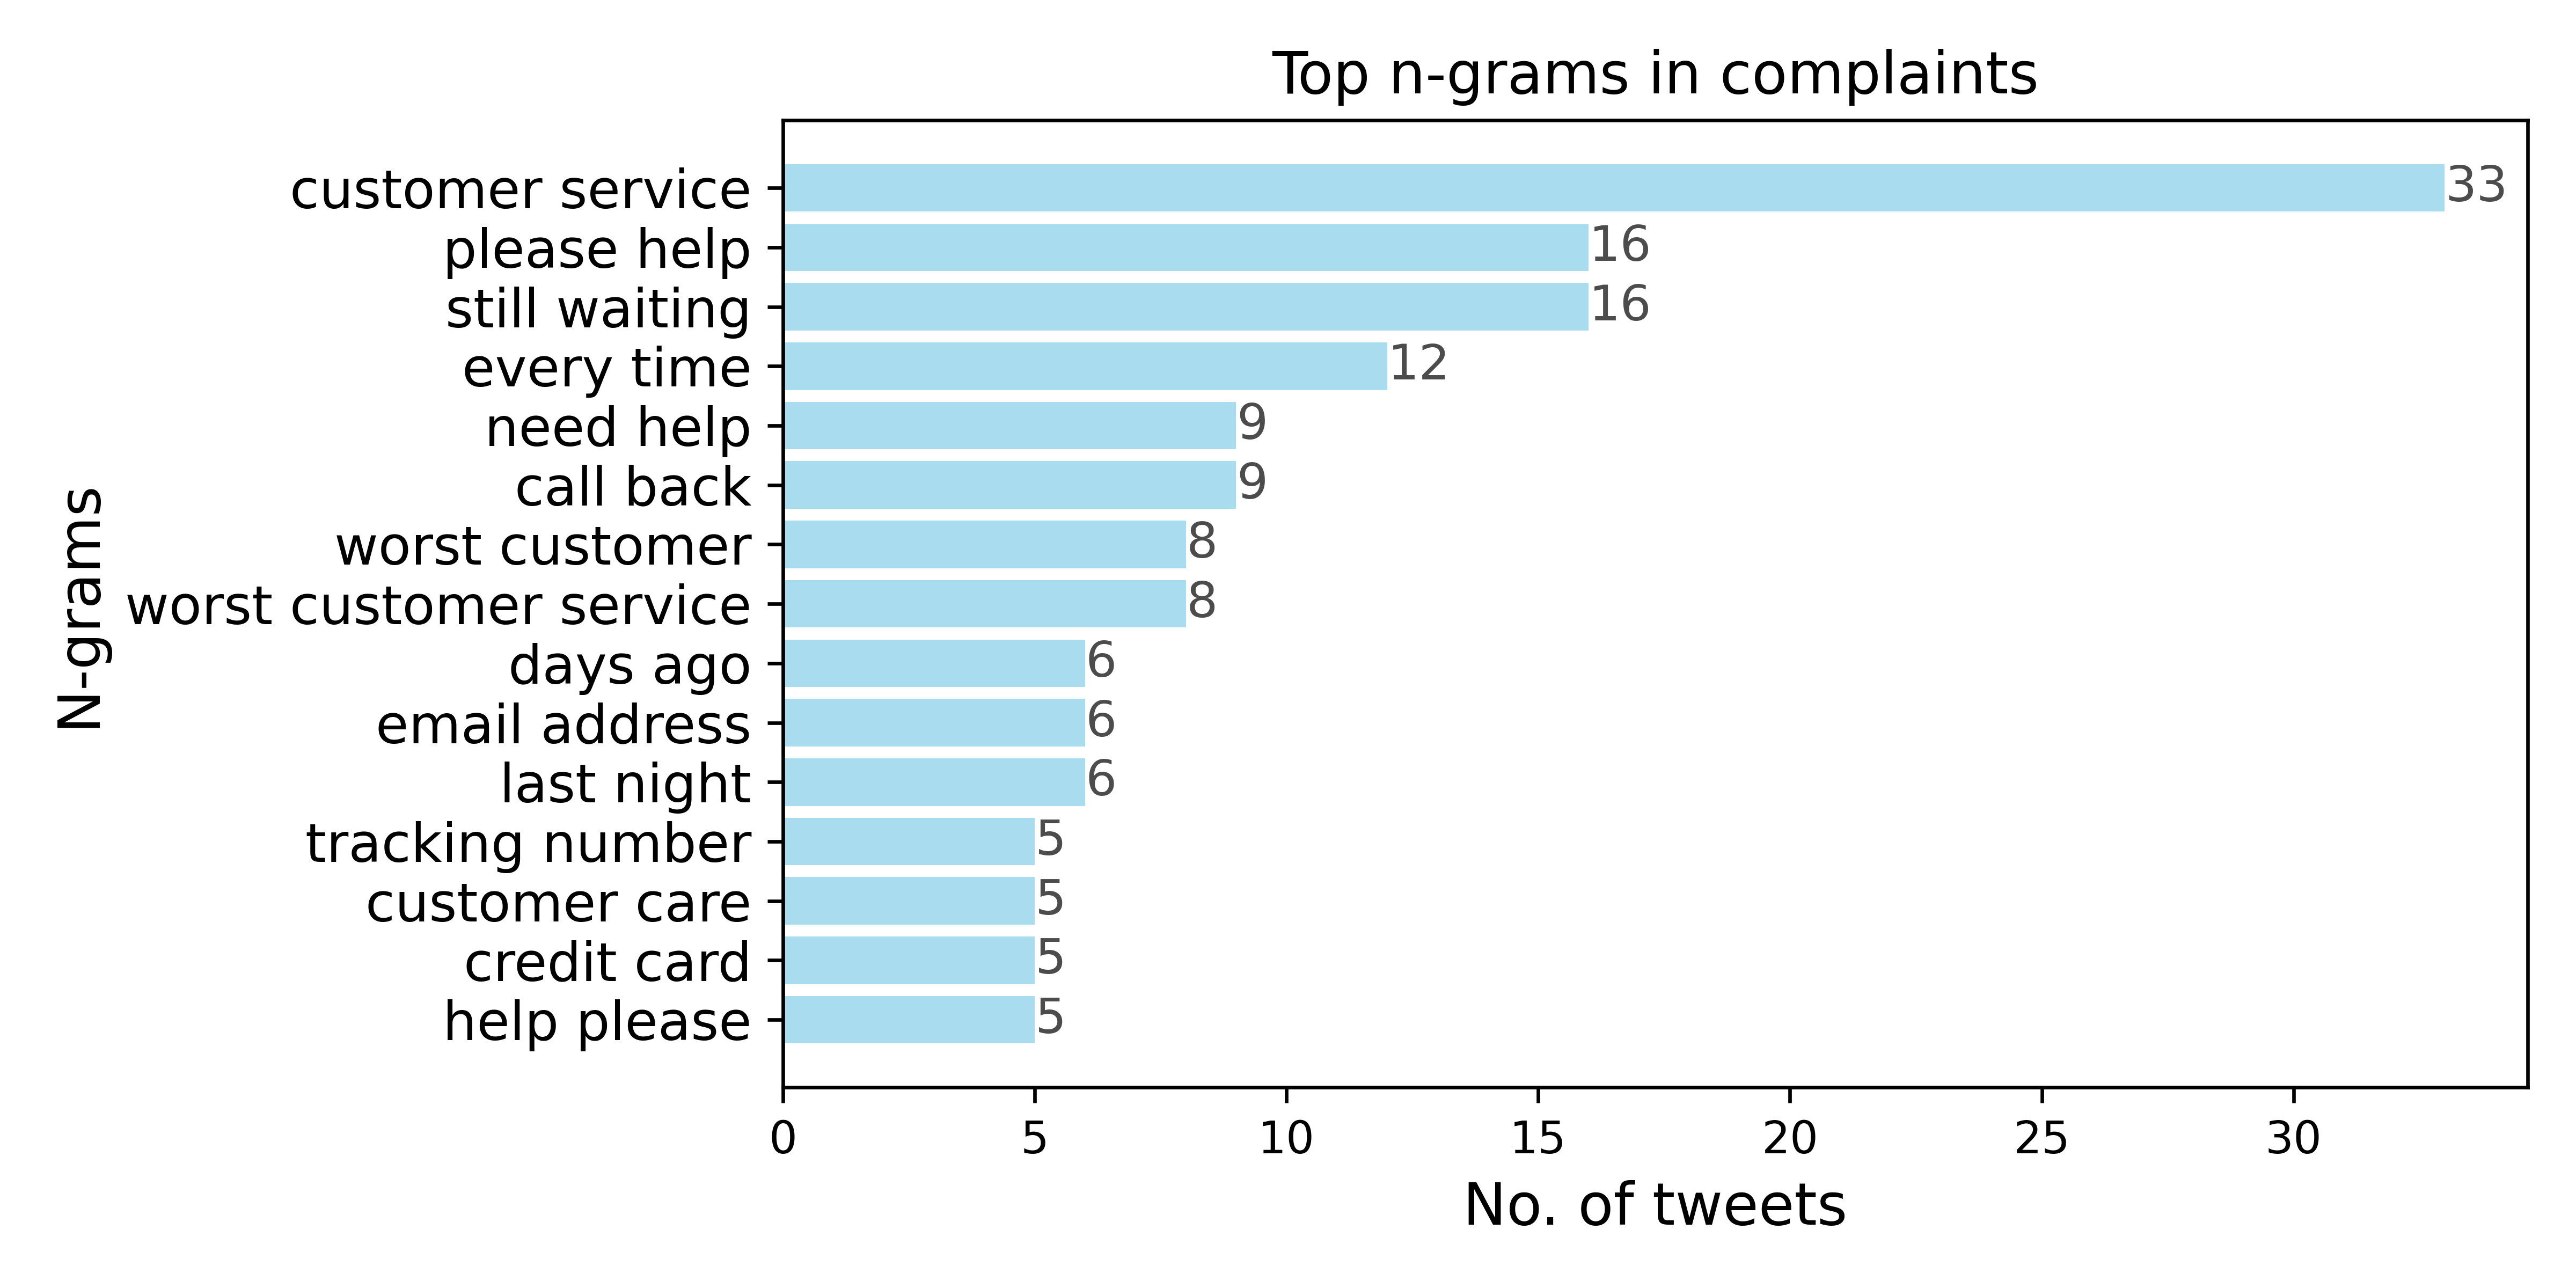
\includegraphics[width=\linewidth]{figures/top_ngram_horiz_bar.png}
        \caption{Top n-grams}
        \label{fig: top_ngrams}
    \end{subfigure}
    \hfill
    \begin{subfigure}{0.49\textwidth}
        \centering
        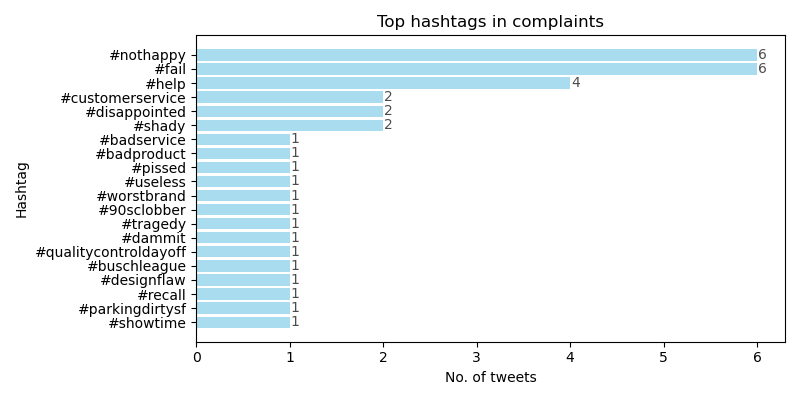
\includegraphics[width=\linewidth]{figures/top_hash_horiz_bar.png}
        \caption{Top hashtags}
        \label{fig: top_hashtags}
    \end{subfigure}
    \caption{Top n-grams(excl. unigrams) and hashtags in the complaint tweets.}
    \label{fig: top_ngrams_hashtags}
\end{figure}

\subsection{Linguistic analysis}
Delving deeper into the language used in Twitter complaints, the top phrases are analysed by extracting the top 15 n-grams. As depicted in Figure \ref{fig: top_ngrams}, common phrases used are meant to convey anticipation of resolution (such as "please help" and "need help"), express frustration (like "still waiting," "worst customer service," and "call back"), and pertain to broader customer service themes (for instance, "tracking number" and "customer care"). To elaborate further, sample tweets with these phrases are shown below. They showcase various characteristics previously discussed, including instances of Face Threatening Acts, feelings of betrayal, altruistic behaviour (warning others), as well as elements like sarcasm. These findings align with the definition of a complaint and the intentions of the speaker as outlined in previous chapters.\\

\textbf{Examples for expectation of rectification}
\begin{quote}
    \textit{"hey chrysler cares i'm the one with the 2011 200 \textbf{need help} with the heating . inside the car it's really strange"}
\end{quote}
\begin{quote}
    \textit{"can someone \textbf{please help} me ? i've already sent a dm ."}
\end{quote}
\textbf{Examples for expression of frustration}
\begin{quote}
    \textit{"\textbf{worst customer service} experience with <user> <user> <user> . never been treated with such contempt"}
\end{quote}
\begin{quote}
    \textit{"on hold with <user> an hour just to get told to \textbf{call back} another day . hell yeah"}
\end{quote}
\begin{quote}
    \textit{"\textbf{worst customer service} to-date <user> in greensboro off wendover . avoid this place and let's show them we have other choices . \#otherchoices"}
\end{quote}

Examination of the hashtags within the complaint tweets indicates that hashtags are predominantly used as a means of conveying frustration, as illustrated in Figure \ref{fig: top_hashtags}. Hashtags such as \texttt{\#nothappy}, \texttt{\#fail}, and \texttt{\#disappointed} serve as examples. Consequently, in addition to being used as a medium for expressing dissatisfaction, these hashtags also communicate negative sentiments. Apart from these particular types of hashtags, various brand-specific or product-specific hashtags are used as well. As per Twitter\footnote{\url{https://help.twitter.com/en/using-twitter/how-to-use-hashtags#}}, users utilize the symbol "\#" (hashtag) preceding a keyword or phrase significant to the context in their tweet to classify those tweets, facilitating their visibility in Twitter searches. Clicking or tapping on a hashtagged term within any message reveals additional Tweets containing the same hashtag. Hashtags can be inserted at any point within a Tweet. Frequently, words marked with hashtags that attain significant popularity transform into trending topics. \\

However, focusing solely on the volumes, the presence of hashtags within the dataset, particularly in the context of complaints, is relatively low. Out of a total of 459 tweets, only 149 complaint tweets incorporate hashtags, constituting roughly 12\% of all complaint-related tweets. When excluding random tweets and replies, the tweets that are not complaints containing hashtags amount to only 67 instances. On average, tweets with at least one hashtag feature 1.56 hashtags. While the inclusion of hashtags may offer some assistance to the predictions by the models, their overall impact on the fine-tuning process could be quite limited due to their low prevalance in the dataset.\\

\subsection{Sentiment analysis}
\begin{figure}[htb]
    \centering
    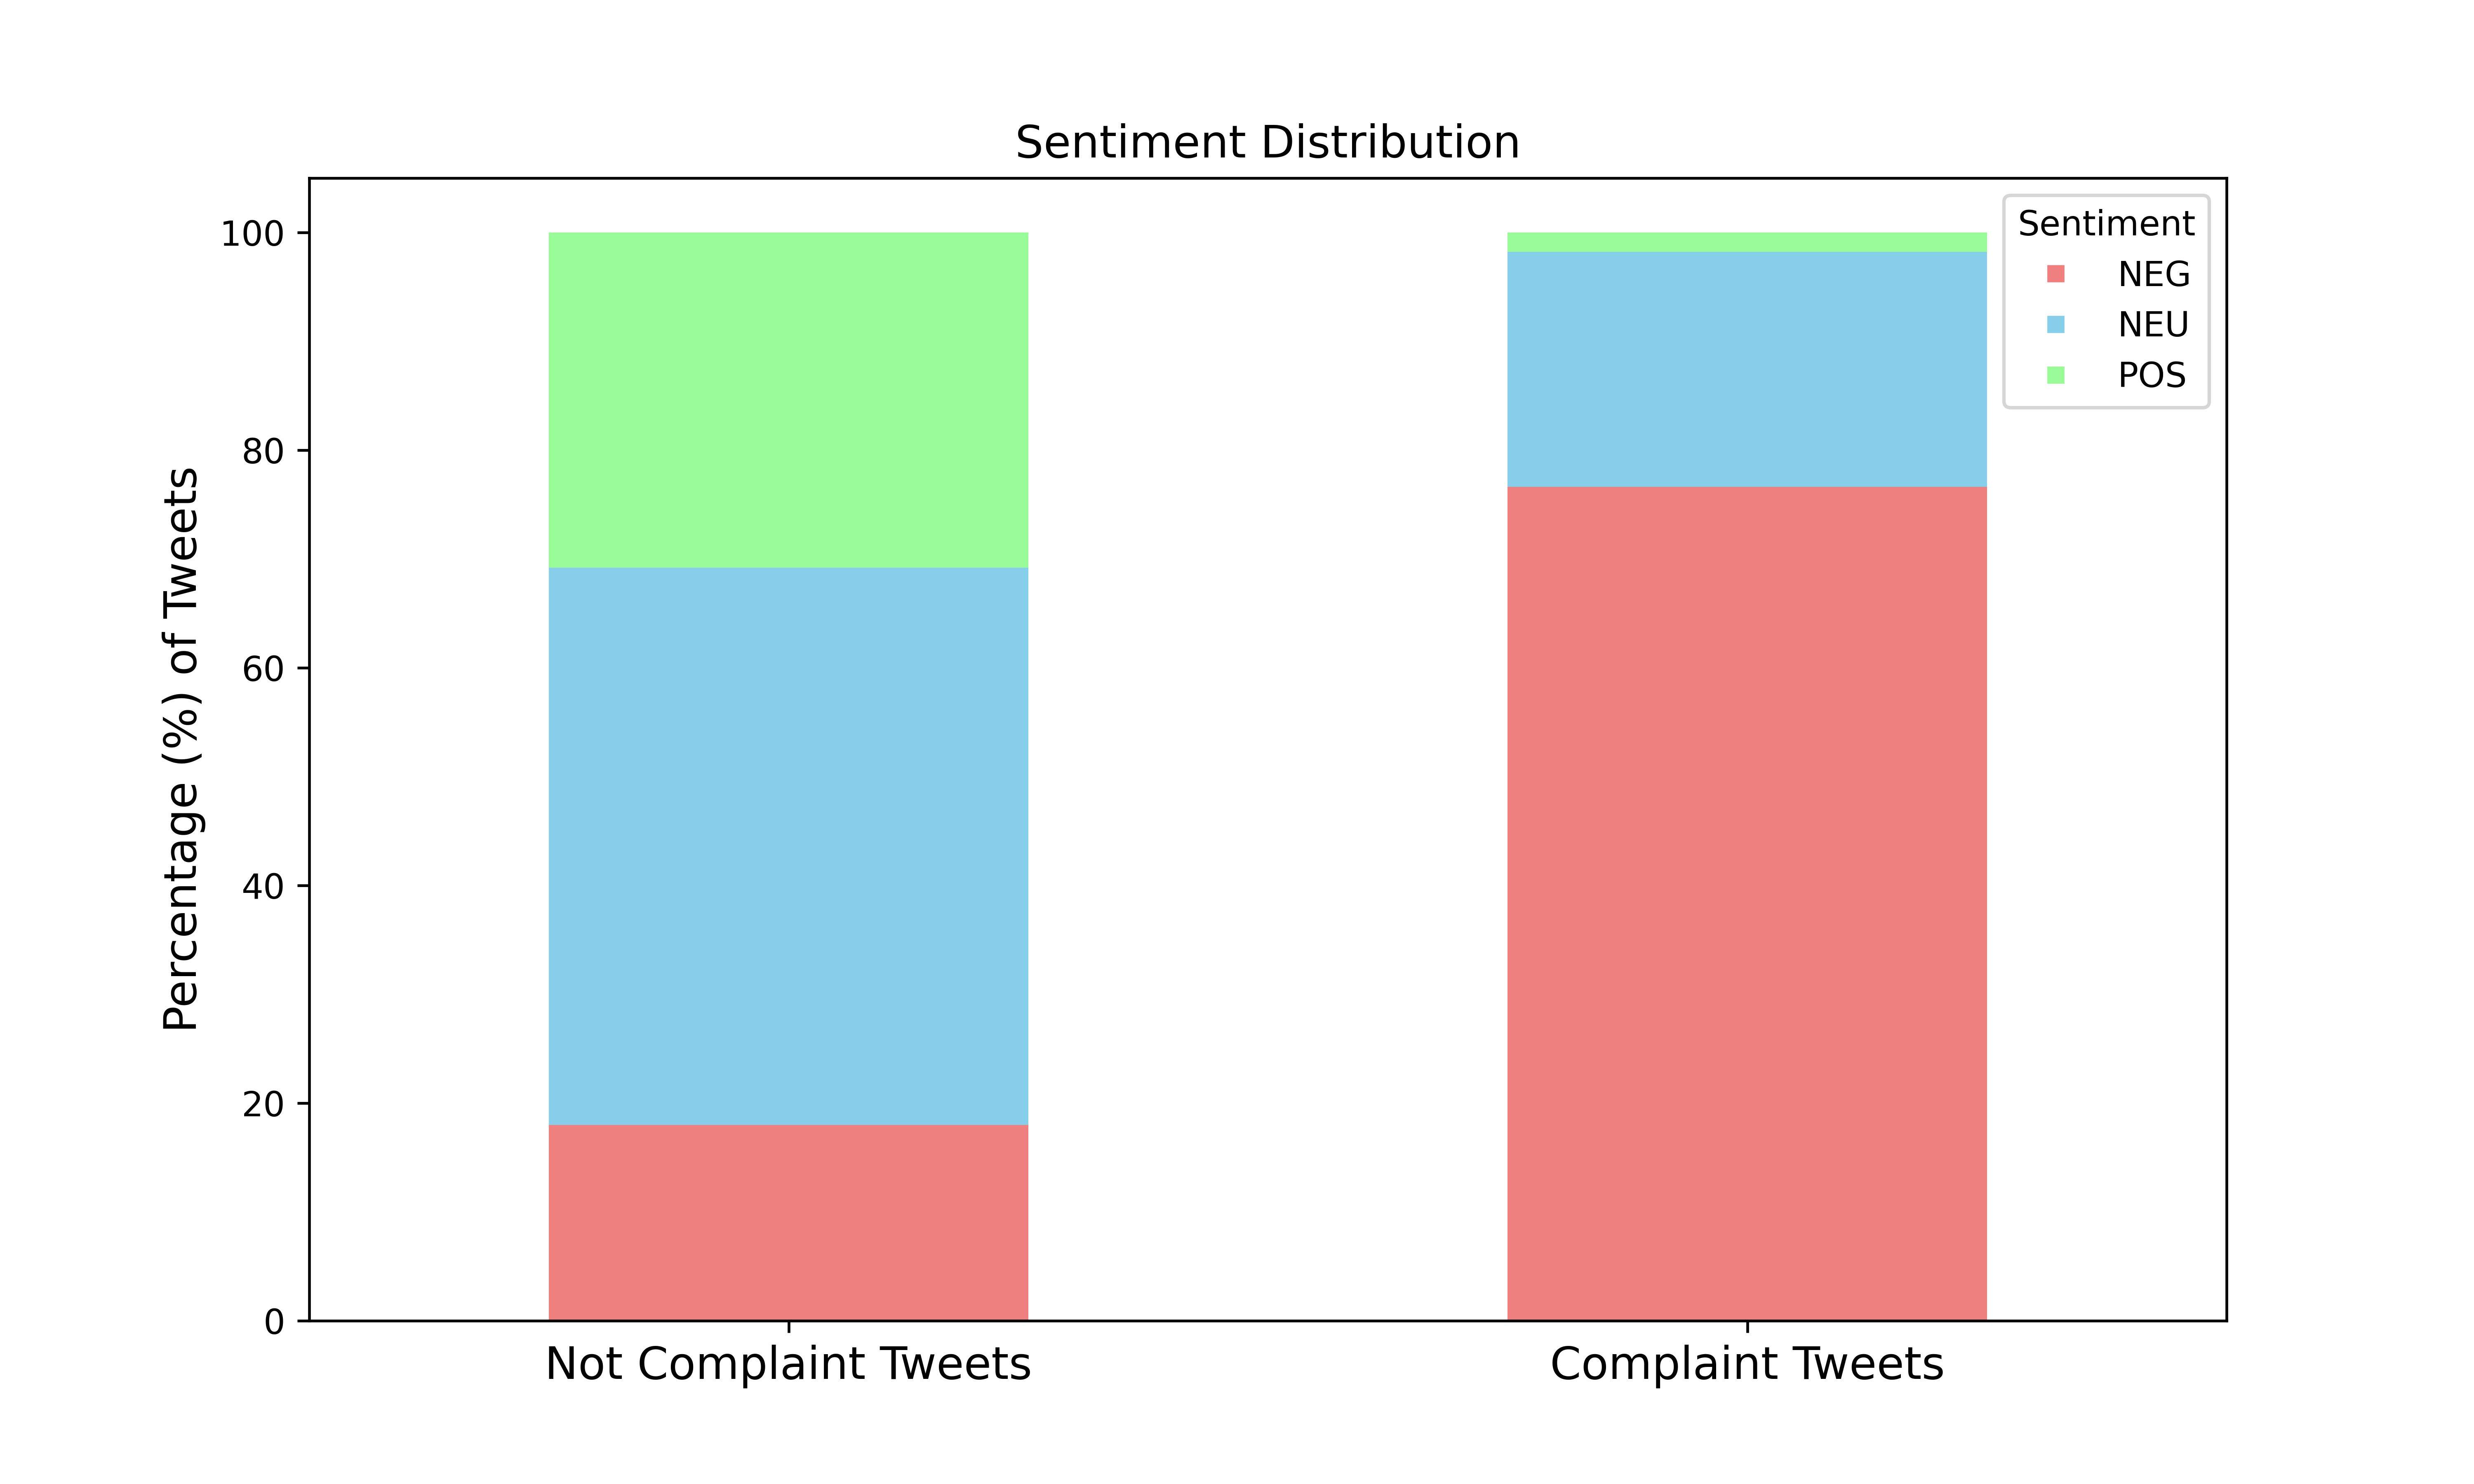
\includegraphics[width=9cm]{figures/sentiment.png}
    \vspace*{-3mm}
    \caption{Distribution of positive, negative and neutral sentiments in the tweets.}
    \label{fig: sentiment}
\end{figure}

The act of complaining typically involves conveying a sense of negativity. The outcome of sentiment analysis, conducted using pysentimiento's sentiment analysis tool \cite{perezPysentimientoPythonToolkit2021}, is depicted in Figure \ref{fig: sentiment}. As expected, the majority of complaint-related tweets convey some form of negative sentiment, while approximately a quarter of them exhibit a neutral sentiment. A couple of examples of such neutral sentiment tweets are as follows: \textit{"anyone know what's up with the geforce 500 series 580 gpx driver 275.33"} and \textit{"hi m order is 913181 did you revise the money ? if you did .. how about the shipping ?"}. These instances appear to involve raising a complaint while simultaneously posing a question that doesn't overtly express negative sentiment. While an undercurrent of dissatisfaction is evident, the situation has not escalated to the point requiring language which explicitly expresses negative sentiment. For tweets that are not complaints, the majority of them express neutral or positive sentiments.

\subsection{Key statistics}
\begin{table}[htbp]
    \captionsetup{font=small}
    \small
    \centering
    \begin{tabularx}{\textwidth}{|l|X|X|X|X|}
        \hline
        \rowcolor[gray]{0.7}
        \textbf{Statistic}              & \textbf{All Tweets} & \textbf{Complaints} & \textbf{Not Complaints} & \textbf{Random} \\
        \hline
        Number of tweets                & 3,                  & 1232                & 742                     & 1475            \\
        \rowcolor[gray]{0.9}
        Number of unique tweets         & 3395                & 1232                & 737                     & 1427            \\
        \hline
        \hline
        Max tweet length (char.)        & 297                 & 297                 & 266                     & 144             \\
        \rowcolor[gray]{0.9}
        Min tweet length (char.)        & 1                   & 7                   & 6                       & 1               \\
        Mean tweet length (char.)       & 77.8                & 96.7                & 70.2                    & 65.8            \\
        \rowcolor[gray]{0.9}
        Median tweet length (char.)     & 79.0                & 98.0                & 68.0                    & 63.0            \\
        Standard Deviation tweet length & 41.4                & 40.5                & 38.9                    & 37.5            \\
        \hline
        \hline
        Total number of tokens          & 55169               & 24260               & 10839                   & 20070           \\
        \rowcolor[gray]{0.9}
        No. of unique tokens            & 7937                & 4031                & 2558                    & 4386            \\
        Maximum tokens                  & 57                  & 57                  & 55                      & 39              \\
        \rowcolor[gray]{0.9}
        Minimum tokens                  & 1                   & 2                   & 1                       & 1               \\
        Mean tokens                     & 16.0                & 19.7                & 14.6                    & 13.6            \\
        \rowcolor[gray]{0.9}
        Median tokens                   & 16.0                & 20.0                & 14.0                    & 13.0            \\
        Standard Deviation for tokens   & 8.6                 & 8.4                 & 8.0                     & 8.0             \\
        \hline
        \hline
        Mean punctuation count          & 3.4                 & 3.9                 & 2.7                     & 3.3             \\
        \hline
    \end{tabularx}
    \caption{Statistics of tweets in the dataset.}
    \label{tab: tweets_statistics}
\end{table}

Finally, examining some of the key statistical measures from the tweets dataset in Table \ref{tab: tweets_statistics}, we observe that complaint tweets tend to exhibit a higher average tweet length, both in terms of characters (96.7) and tokens (19.7). In contrast, random tweets and replies have a token count lower by 30\%, while non-complaint tweets possess an average of 14.6 tokens or 25\% fewer than complaint tweets. This disparity may stem from individuals employing diverse linguistic expressions to express their dissatisfaction or disappointment, or to communicate a Face Threatening Act directed at the subject of the complaint.

\section{Experiment set 1 results: Comparision of model performance}
As described in the previous chapter, to compare the performance of the models a nested cross-validation approach was adopted. The cross-validation method finetuned the models using 4 learning rates, $l\:\epsilon\:[1e-5, 5e-6, 5e-5, 3e-5]$ with the best-performing model based on the F1 score being selected for the testing for each iteration of the outer loop. \\

\subsection{Best predictive performance}
The best-performing model was found to be BERTweet with a mean F1 score of 0.908 (sd: $\pm$0.01) and accuracy of 0.934 (sd: $\pm$0.01) as shown in Table \ref{tab: model_mean_metrics}. BERTweet being pre-trained on a corpus of 850M tweets seems to give it a significant advantage in capturing the nuances of social media posts including informal language, typographic errors, use of slang and expressive lengthening and more specific characteristics of tweets such as the use of shorter messages, abbreviations and hashtags. RoBERTa was the next best performing model with an F1 of 0.879 (sd: $\pm$0.03) and an accuracy of 0.914 (sd: $\pm$0.02). It was followed by BERT base and DistilBERT with F1 scores of 0.865 (sd: $\pm$0.02) and 0.863 (sd: $\pm$0.02) respectively. \\

Table \ref{tab: model_mean_metrics} also includes the prediction metrics sourced from \cite{jin_complaint_2020}, enclosed within '[ ]', which serves as the established baseline performance for this task. Despite the variation in nested cross-validation configuration, as outlined in the preceding chapter, a level of preliminary comparison becomes feasible. In terms of F1 scores, RoBERTa shows marginal improvement, while BERT base and ALBERT perform slightly worse. However, overall BERTweet provides the best predictive results for this task when compared to the baseline.\\

\begin{table}[htbp]
    \centering
    \small % Set font size to \small
    \begin{tabularx}{\textwidth}{|X|X|X|X|X|X|}
        \hline
        \rowcolor[gray]{0.7}
        \textbf{Model}                         & \textbf{Accuracy} & \textbf{Precision} & \textbf{Recall} & \textbf{F1}    & \textbf{ROC AUC} \\
        \hline
        AlBERT base v2                         & 0.879 [0.859]     & 0.845 [0.848]      & 0.811 [0.846]   & 0.827 [0.846]  & 0.864            \\
        \rowcolor[gray]{0.9}
        \(\uparrow\) BERTweet base             & \textbf{0.934}    & \textbf{0.897}     & \textbf{0.920}  & \textbf{0.908} & \textbf{0.931}   \\
        BERT base uncased                      & 0.905 [0.88]      & 0.878  [0.871]     & 0.854  [0.873]  & 0.865 [0.87]   & 0.894            \\
        \rowcolor[gray]{0.9}
        \(\downarrow\) BERT tiny \vspace{10pt} & 0.772             & 0.701              & 0.627           & 0.662          & 0.739            \\
        DistilBERT base uncased                & 0.903             & 0.872              & 0.860           & 0.863          & 0.894            \\
        \rowcolor[gray]{0.9}
        MobileBERT uncased                     & 0.887             & 0.843              & 0.843           & 0.841          & 0.877            \\
        RoBERTa base                           & 0.914 [0.876]     & 0.886 [0.866]      & 0.873 [0.869]   & 0.879 [0.866]  & 0.905            \\
        \hline
    \end{tabularx}
    \caption{Mean prediction performance metrics for all models after nested cross-validation for finetuning and testing. The highest scores are in bold. \(\uparrow\) is the best performing and \(\downarrow\) is the worst performing model. Where available, numbers in '[ ]' are the results from \cite{jin_complaint_2020}.}
    \label{tab: model_mean_metrics}
\end{table}

\subsection{Performance of 'lightweight' models}
Examining the models characterized as lightweight based on their architecture and parameter count, DistilBERT emerges as the top performer, achieving an F1 score of 0.863 (sd: $\pm$0.02). MobileBERT and ALBERT follow suit with F1 scores of 0.841 (sd: $\pm$0.02) and 0.827 (sd: $\pm$0.05) respectively. On the other hand, BERT Tiny, the smallest model employed in the experiments, exhibits a notable performance gap, achieving only an F1 score of 0.662 (sd: $\pm$0.04), which is lower by 27.6\% in comparison to BERTweet. This points to a likely and significant performance penalty in this case from the reduced model size although it is expected to perform better in the context of a knowledge distillation teacher \cite{turcWellReadStudentsLearn2019}, something that has not been tested here.\\

\begin{figure}[htb]
    \centering
    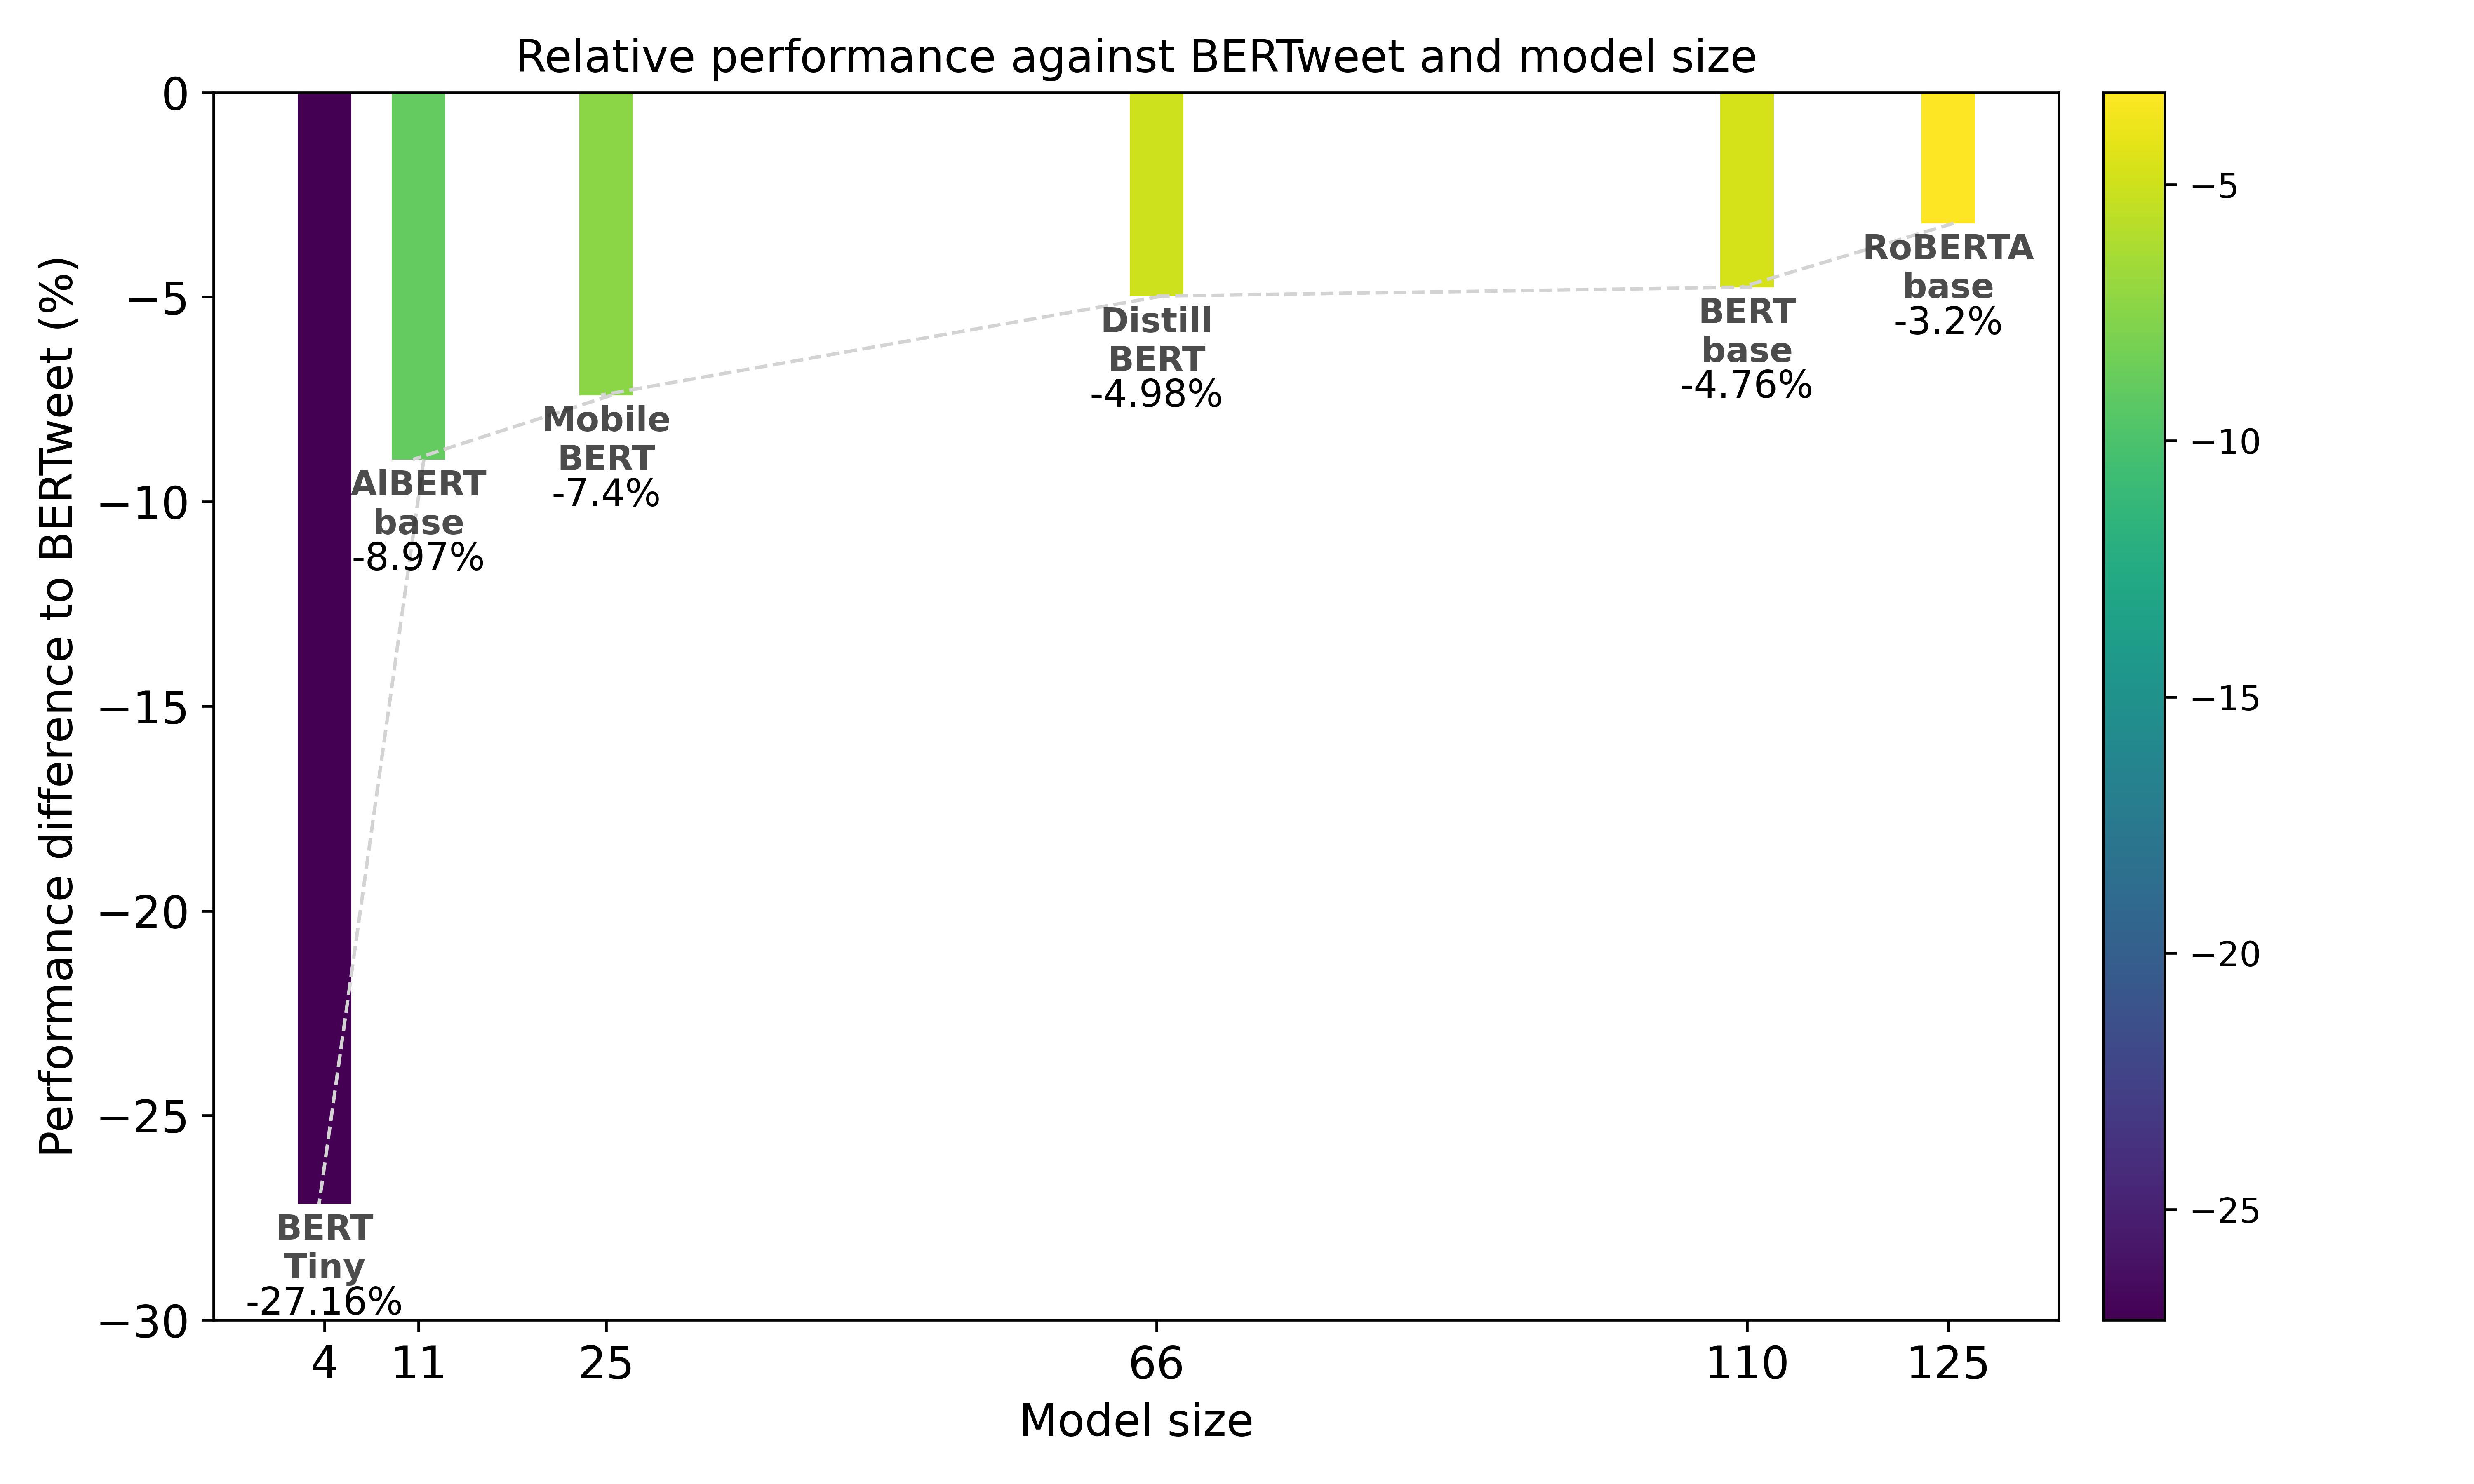
\includegraphics[width=9cm]{figures/model_size_vs_perf.png}
    \vspace*{-3mm}
    \caption{Relative performance of models against BERTweet and model sizes based on F1. BERTweet's model size is 110M.}
    \label{fig: model_size_vs_perf}
\end{figure}

Figure \ref{fig: model_size_vs_perf} displays the relative variance in model performance when compared to BERTweet based on F1, alongside the corresponding model sizes or the number of parameters. Notably, ALBERT and MobileBERT exhibit relatively lower performance discrepancy of only 8.9\% and 7.4\%, considering the model sizes are lower significantly by 90\% and 77\% respectively. Similarly, DistilBERT demonstrates a performance deficit of merely 4.9\%, akin to that of BERT base, while having a 44\% reduction in model size. This correlation suggests that the knowledge distillation compression technique applied during the pretraining phase could be playing a pivotal role in enhancing DistilBERT's predictive capabilities \cite{sanhDistilBERTDistilledVersion2020}.

\subsubsection{Analyis of finetuning and inference time}
Next, analysing the time required for inference and training or in the scope of the experiments, finetuning we fine 
\begin{figure}[htbp]
    \centering
    \captionsetup{font=small}
    \begin{subfigure}{0.49\textwidth}
        \centering
        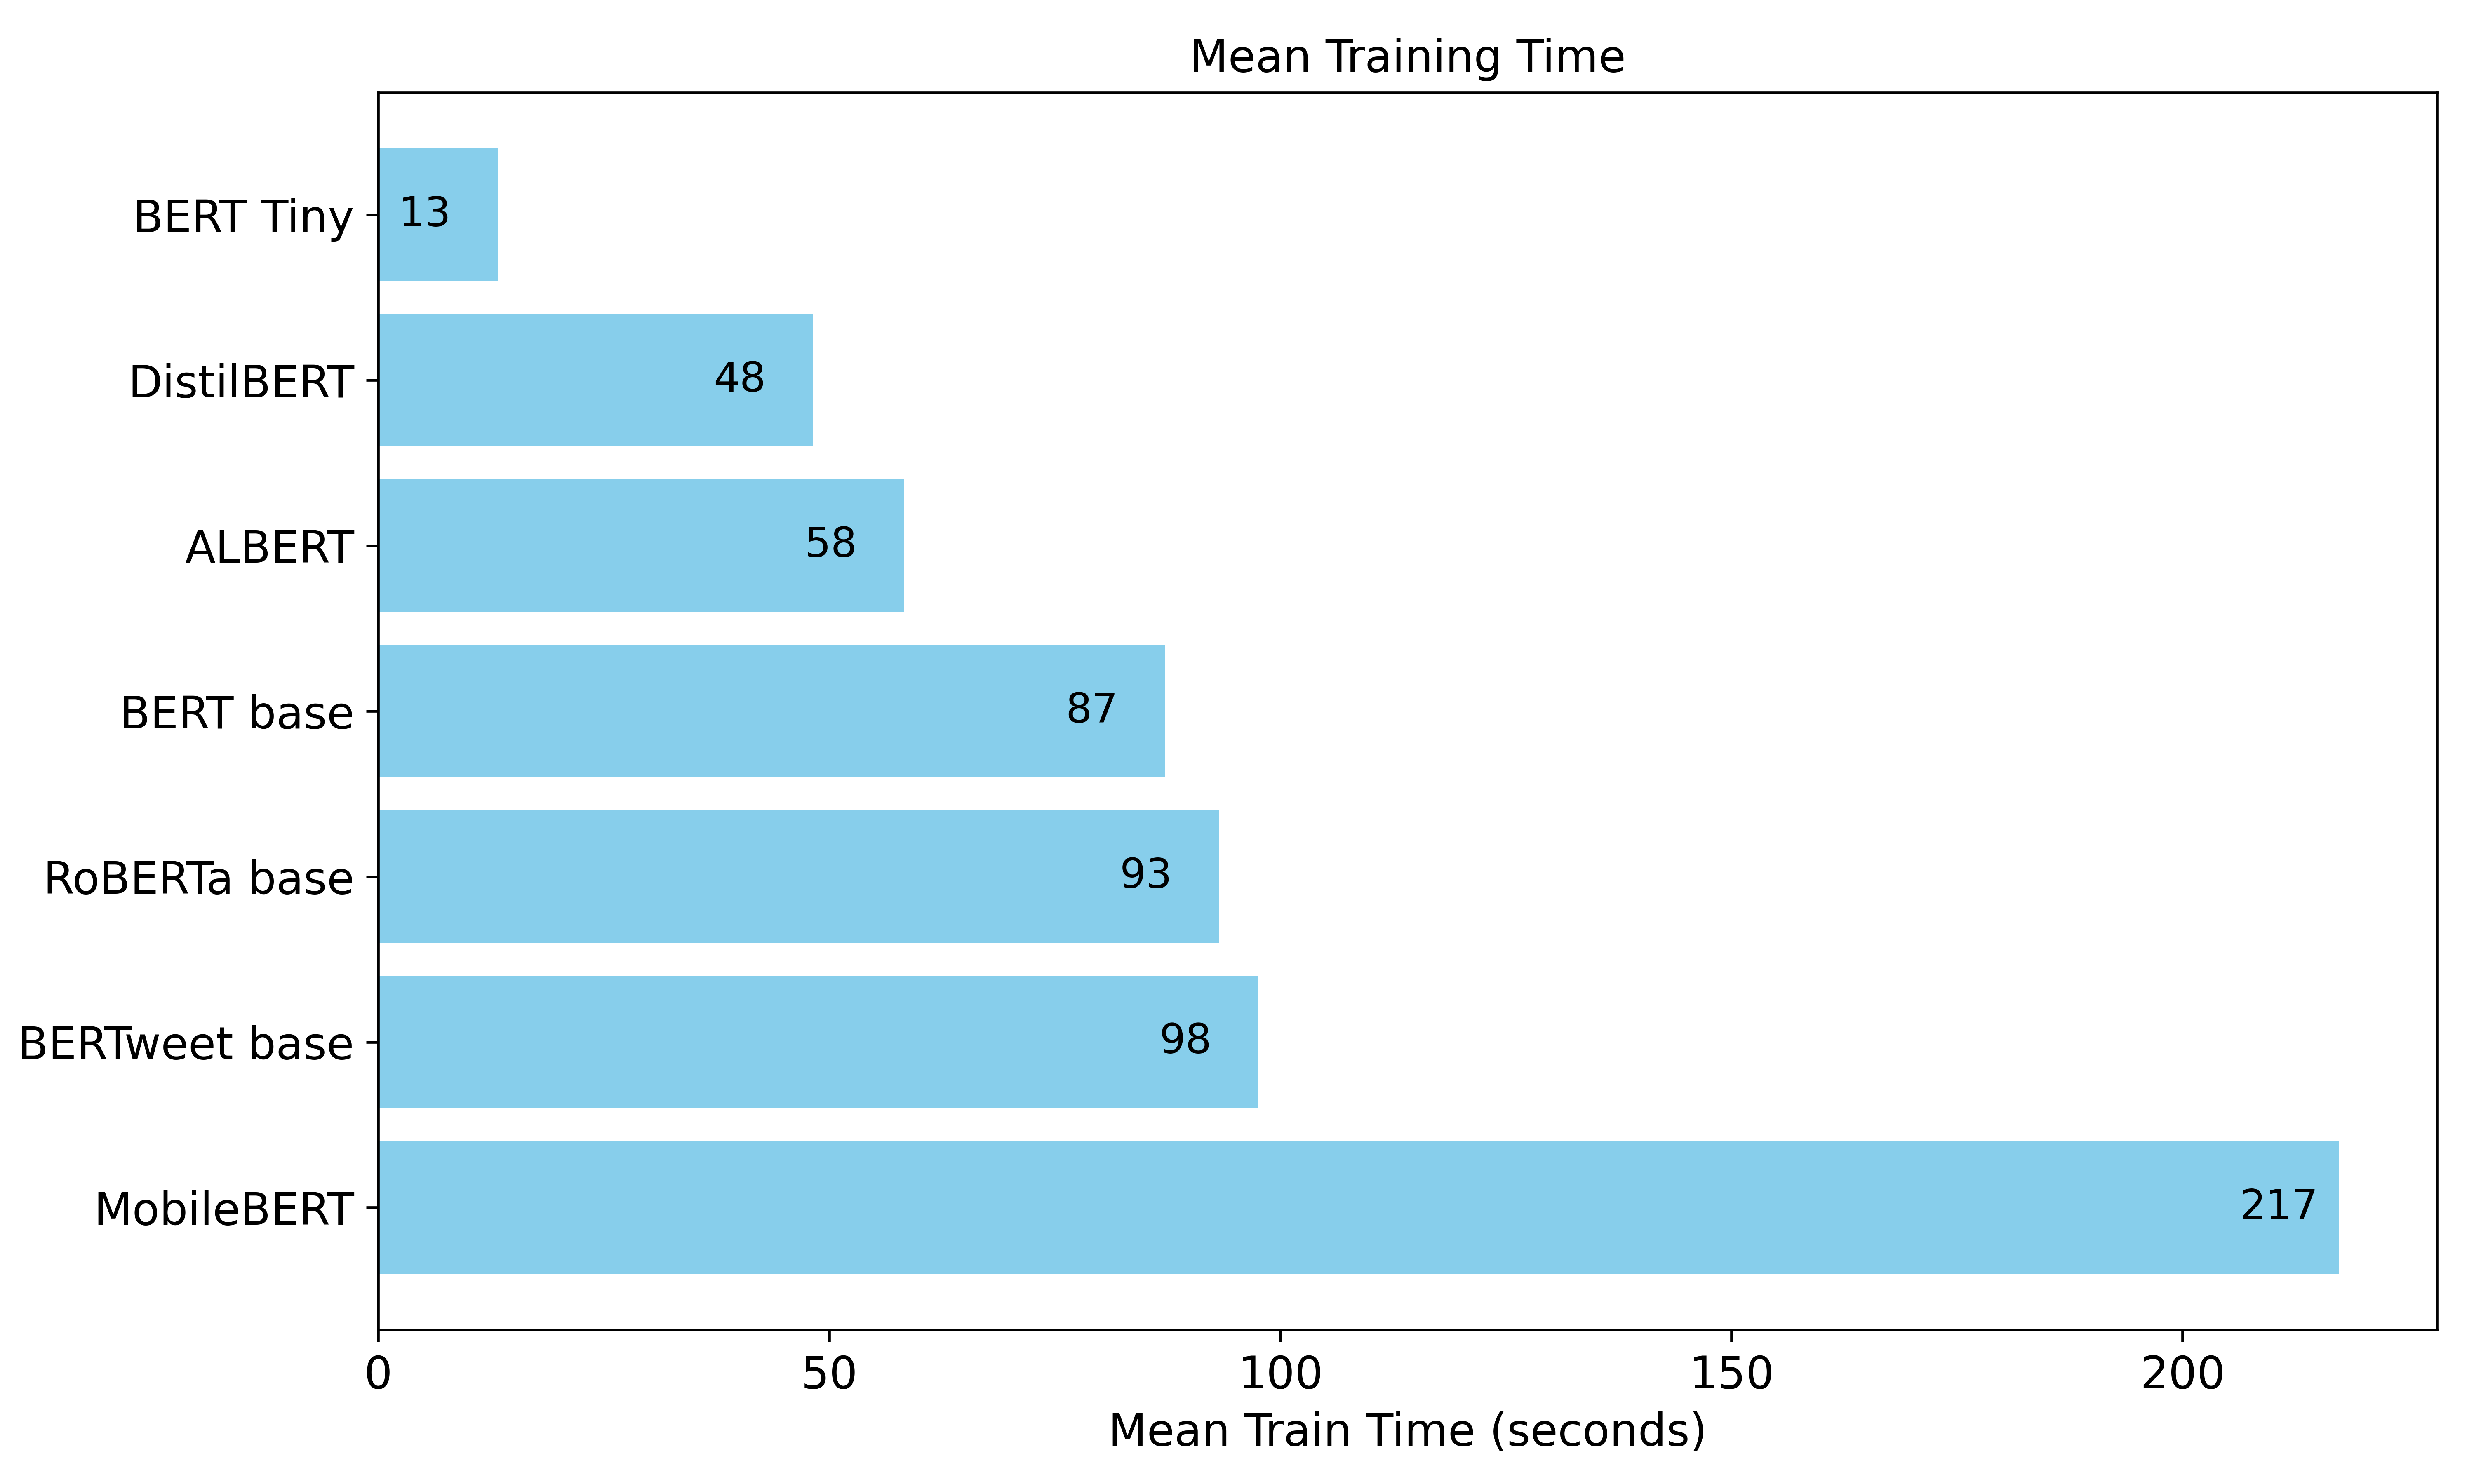
\includegraphics[width=\linewidth]{figures/mean_train_time.png}
        \caption{Mean training time.}
        \label{fig: mean_train_time}
    \end{subfigure}
    \hfill
    \begin{subfigure}{0.49\textwidth}
        \centering
        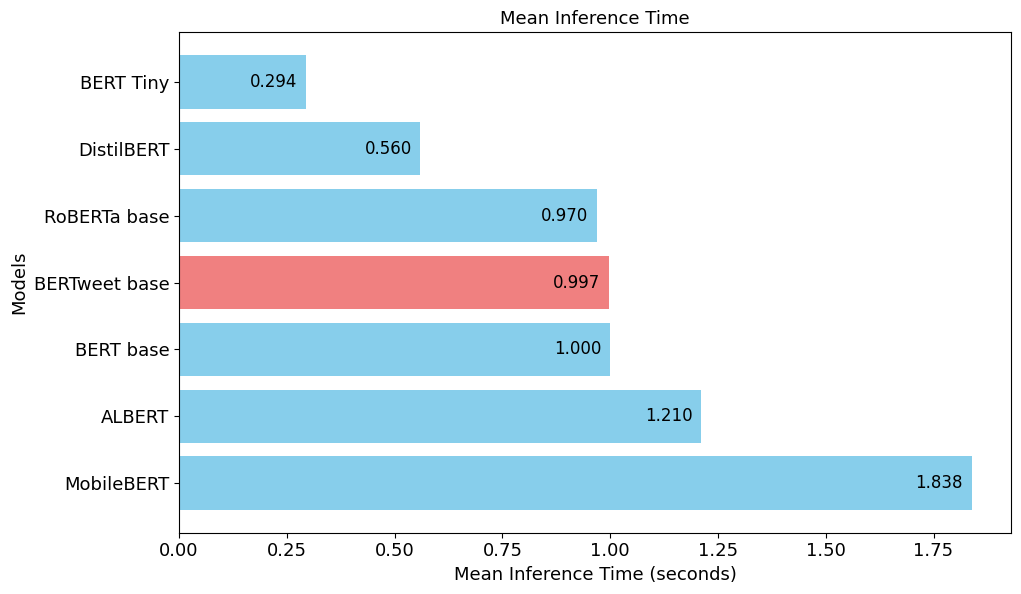
\includegraphics[width=\linewidth]{figures/mean_inference_time.png}
        \caption{Mean inference time}
        \label{fig: mean_inf_time}
    \end{subfigure}
    \caption{Mean time taken for finetuning and inference during experiments set 1.}
    \label{fig: mean_time_taken}
\end{figure}

\subsection{Deep-dive into the results}
**TO UPDATE**



\section{Experiment set 2 results: Cross-domain results}
**TO UPDATE**